%------------------------------------------------------------------------
%Editar Diplomado
\hypertarget{cv:GestionarTray}{\section{Gestionar Trayectorias}} \label{sec:GestionarTray}

	Esta funcionalidad le permitirá las acciones necesarias para controlar las trayectorias pertenecientes a un caso de uso y visualizarlos en una tabla en el proyecto sobre el que se está operando y solicitar el registro de una nueva.

		\subsection{Procedimiento}

			%Pasos de procedimiento
			\begin{enumerate}
			
			\item Oprima el botón \IUTray{} de algún registro existente de la pantalla \ref{fig:GestionarCU} ''Gestionar Casos de Uso''.
	
			\item Se mostrará la pantalla \ref{fig:GestionarTrayectorias} ''Gestionar Trayectorias''.

			%Pantalla
			\begin{figure}[htbp!]
				\begin{center}
					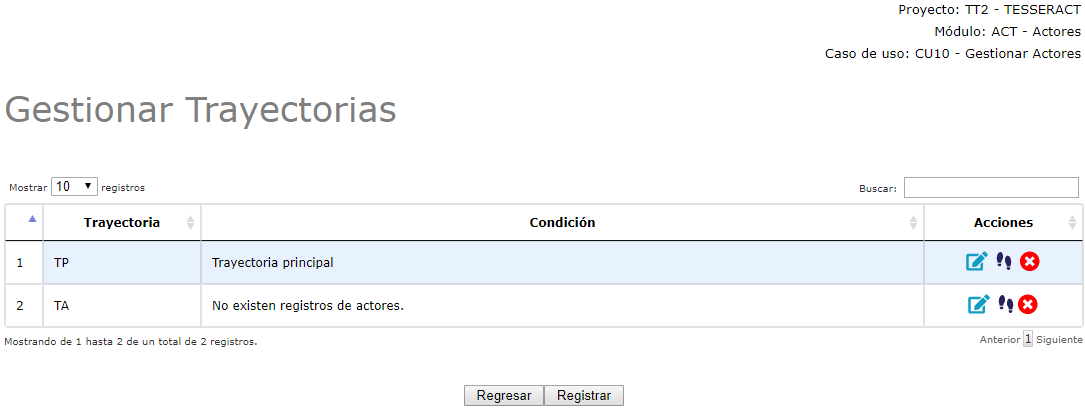
\includegraphics[scale=0.6]{roles/lider/casosUso/trayectorias/pantallas/IU6-1-1gestionarTray}
					\caption{Gestionar Trayectorias}
					\label{fig:GestionarTrayectorias}
				\end{center}
			\end{figure}
		
				\item Seleccione la operación que desea realizar:
			
			Para (\hyperlink{cv:registrarTray}{Registrar}) dé clic en el botón \IURegistrar.
			
			Para (\hyperlink{cv:modificarTray}{Modificar}) dé clic en el icono \IUEditar{} de alguna trayectoria ya registrada.
			
			Para (\hyperlink{cv:eliminarTray}{Eliminar}) dé clic en el icono \IUBotonEliminar{} de alguna trayectoria ya registrada.
			
			Para (\hyperlink{cv:GestionarPasos}{Gestionar Pasos}) dé clic en el icono \IUPasos de alguna trayectoria ya registrada.
			
			\end{enumerate}